\def \currentAuthor {Kevin Glatz}
\newpage


\section{Verkablung}

Die Verkablung der einzelnen Module ist aus verschiedenen Gründen wichtig. Zum einen brauch jedes Modul genügend Strom um seine Aufgabe zu erfüllen, gleichzeitig würde es aber ohne die Erdung zu einem Kurzschluss kommen. Des weiteren ist es wichtig das die Module Daten auslesen und weitersenden können

\subsection{Aufbau}

(bild einfügen)

In Abbildung x können wir nun den Arduino und das Breadboard sehen.  Dort kann man direkt die drei Farben erkennen die jeweils für Stromzufuhr (blau), Datenauslesung (grün) und Erdung (braun) stehen.

(bild mit stromfluss einfügen)

Hier sieht man wie der Strom im Breadboard fließt. Das heißt wenn man in der Untersten Reihe das Board mit 5 Volt versorgt sind alle weiteren Steckplätze verwendbar. Wichtig hierbei ist, dass das Kabel für die Stromzufuhr auch auf der richtigen Reihe platziert wurde. Das erkennt man bei dieser Leiterplatte an dem Plus und Minus Zeichen Plus steht hierbei für Strom und Minus für die Erdung.

Falls man das Falsch verkabelt funktioniert das Modul nicht, es werden allerdings keine Schäden angerichtet


(Bild mit analog und digitalwerten einfügen)

Der Arduino hat zwei Möglichkeiten Daten auszulesen. Einmal spricht man hier von digitaler und analogen Datenauslesung. (internet suche) Digitale Werte bedeutet hier allerdings nur das der ausgelesene Wert als 0 oder 1 abgespeichert werden kann, analoge Daten sind bei diesem Punkt anders, da diese einen Wert zwischen 0 und x haben können (zitat)

\section{Programmierung}

Um die Daten der einzelnen Sensoren verwenden zu können, müssen diese ausgelesen und sinnvoll wiedergegeben werden. Nur sobald die Sensoren richtig Programmiert und verkabelt sind, kriegt man lesbare Information. Diese können anschließend weiter interpretiert und verwendet werden. 

Die verwendeten Sensoren:

\begin{itemize}
	\item DHT11
	\item CCS811
	\item Hebel
	\item Servo SG90
	\item photocell
\end{itemize}


\subsection{DHT11 \& CCS811}

Für den DHT 11 sowie dem CCS811 gibt es eine von Adafruit frei verwendbare Bibliothek. Mithilfe von dieser kann man ein Objekt erstellen und es mithilfe diesem Objektes die Momentane Temperatur/Luftfeuchtigkeit auslesen.


	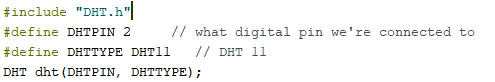
\includegraphics[width=1\linewidth]{../Bilder/Programmierung/define(DHTCCS)}



Das \#include fügt die Klasse in unser Projekt ein und erlaubt es uns das Objekt dht sowie ccs zu erstellen.

Das \#define legt des weiteren fest, dass relevante Daten, im Falle des DHT Moduls, von Pin 2 kommen. 


	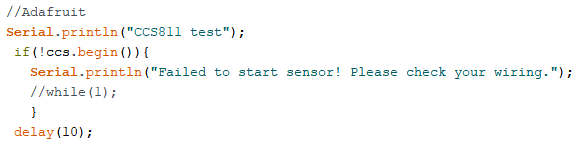
\includegraphics[width=1.2\linewidth]{../Bilder/Programmierung/setup(CCS)}



Die Setup Funktion, wird für einmalige Dinge wie die Kalibrierung, dem Starten des Serial Monitors oder der Verbindung mit dem Raspberry verwendet. Der CO2 Sensor benötigt das Setup, da es zuerst kalibriert werden muss um die Luftqualität zu messen.

	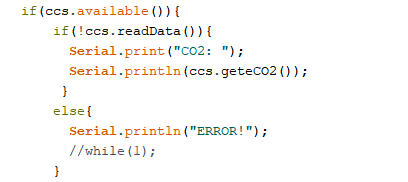
\includegraphics[width=0.9\linewidth]{../Bilder/Programmierung/loop(DHTCCS)}



Die Loop Funktion, wiederholt sich im vorgegebenen Rhythmus immer wieder und gibt keine Variablen zurück. Dort können werden alle Daten ausgelesen und an das WLAN Modul weitergeschickt bzw. in diesem Fall wird es auf den Serial Monitor ausgegeben.

Die WENN abfrage prüft als erstes ob der CO2 Sensor kalibriert wurde oder nicht. Falls es gelungen sein sollte gibt es die Werte mit dem Befehl Serial.println(ccs.geteCO2()); im Serial Monitor aus.

\subsection{Hebel}

Das Joystick bzw. der Hebel konnte direkt abgelesen werden. Wichtig hierbei ist es das man nicht nur eine Achse im Setup verwendet sondern beide, ansonsten kommt es bei dem Loop zu einem Fehler und der Wert der benötigten Achse verändert sich nicht.


\subsection{SG90}

Die vom verwendeten Bibliotheken waren bei der Installierung der Arudino eigenen IDE direkt dabei. Die Servo kontrolliert die Luftzuvor und muss daher Werte vom CCS811 wiederverwenden

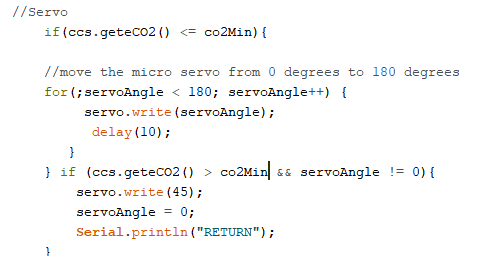
\includegraphics[width=1\linewidth]{../Bilder/Programmierung/loop(SG)}

Die If Abfrage prüft ob CO2 einen Mindestwert (co2Min) unterschreitet. Falls das passiert  wird eine Schleife ausgeführt die den Servo 180° dreht. Diese 180° würde die Lüftungsklappe aufhalten. Falls der CO2 Wert wieder in einem akzeptablen Bereich liegt und die Position des Motors nicht null beträgt, wird die zweite Schleife aktiviert die den Motor zur Position 0 zurückbringt 


\subsection{photocell}


